\documentclass[conference]{IEEEtran}

\usepackage[spanish]{babel}
\usepackage[utf8]{inputenc}
\usepackage{amsmath}
\usepackage{graphicx}
\usepackage[colorinlistoftodos]{todonotes}
\usepackage{tikz}
\usepackage{url}
\usepackage{multicol}
\usepackage{csquotes}
\usepackage{mathtools}
\usepackage{float}
\usetikzlibrary{shapes, shadows, arrows}
\pagenumbering{arabic}
\usepackage{lastpage}
\usepackage{fancyhdr}
\pagestyle{fancy}
\fancyhf{}
\rfoot{Página \thepage \hspace{1pt} de \pageref{LastPage}}


\DeclareMathOperator{\diag}{diag}


\begin{document}
    

\title{Modelado SEIR del COVID-19 y sus dinámicas}

\author{Rafael Mejía Zuluaga - rmejiaz@unal.edu.co}

\maketitle


\section{Introducción}

El presente documento es una réplica del artículo \textit{SEIR modeling of the
COVID-19 and its dynamics}. En este se simula el modelo propuesto por los autores 
y se realiza un análisis de bifurcaciones.

\section{Modelo SEIR}

El modelo SEIR clásico parte de un principio fundamental el cual consiste en dividir a
la población total en cuatro grupos diferentes: $S$ (susceptibles), $E$ (expuestos),
$I$ (infectados) y $R$ (recuperados). La idea es que a media que pasa el tiempo, 
todos los individuos de la población van a pertenecer a todos los grupos, siguiendo la 
ruta $S \rightarrow E \rightarrow I \rightarrow R$. Las variables del sistema son
prescisamente la cantidad de personas en cada uno de estos grupos. El modelo también 
parte de la base que la cantidad total de individuos $N$ se mantiene constante (no toma en
cuenta los nacimientos ni las muertes), por lo que la cantidad de personas que salen de
un grupo necesariamente deben entrar a otro de los grupos, y en todo momento se cumple
$N = S + E + I + R$.
\\\\
El modelo propuesto por los autores es una versión ampliada de este modelo, en el cual 
se incluyen dos categorías más: $H$ (hospitalizados) y $Q$ (en cuarentena). Además, se
divide la categoría de infectados en dos grupos: $I_1$ (infecados sin intervención)
e $I_2$ (infectados con intervención).
\\\\
A diferencia del modelo SEIR clásico, en este modelo se tienen dos canales principales,
el primero es $S \rightarrow E \rightarrow I_1 \rightarrow R$ y el segundo
$S \rightarrow Q \rightarrow I_2 \rightarrow H \rightarrow R$. El primer 
caso ilustra el comportamiento natural de una pandemia y equivale al SEIR clásico, 
mientras que el segundo hace referencia a los mecanismos de control impuestos por los
gobiernos tales como cuarentenas y hospitazaciones. Por último, otra diferencia 
importante de este modelo con respecto al SEIR clásico es que en este los individuos
pueden pasar de $R$ nuevamente a $S$, pues se ha demostrado que es posible volver a 
contagiarse después de haber estado infectado y haberse recuperado. A continuación 
se muestra el modelo propuesto:

\begin{equation}   
    \begin{aligned}
    \left\{
        \begin{array}{l} 
        \dot{S} = - \frac{S}{N}\left( {{\beta _1}{I_1} + {\beta _2}{I_2} + \chi E} \right) + {\rho _1}Q - {\rho _2}S + \alpha R
        \\ 
        \dot{ E} = \frac{S}{N}\left( {{\beta _1}{I_1} + {\beta _2}{I_2} + \chi E} \right) - {\theta _1}E - {\theta _2}E
        \\ 
        {\dot{I}}_1 = {\theta _1}E - {\gamma _1}{I_1}
        \\ 
        \dot{I}_2 = {\theta _2}E - {\gamma _2}{I_2} - \varphi {I_2} + \lambda \left( \varLambda + Q \right) 
        \\ 
        \dot{R} = {\gamma _1}{I_1} + {\gamma _2}{I_2} + \phi H - \alpha R
        \\ 
        \dot{H} = \varphi {I_2} - \phi H
        \\ 
        \dot{Q} = \varLambda + {\rho _2}S - \lambda \left( {\varLambda + Q} \right) - {\rho _1}Q 
    \end{array} 
    \right.
    \end{aligned}
\end{equation}

La figura \ref{block_diagram} muestra un diagrama de flujo del modelo con los diferentes canales.

\begin{figure*}[h]
    \centering
    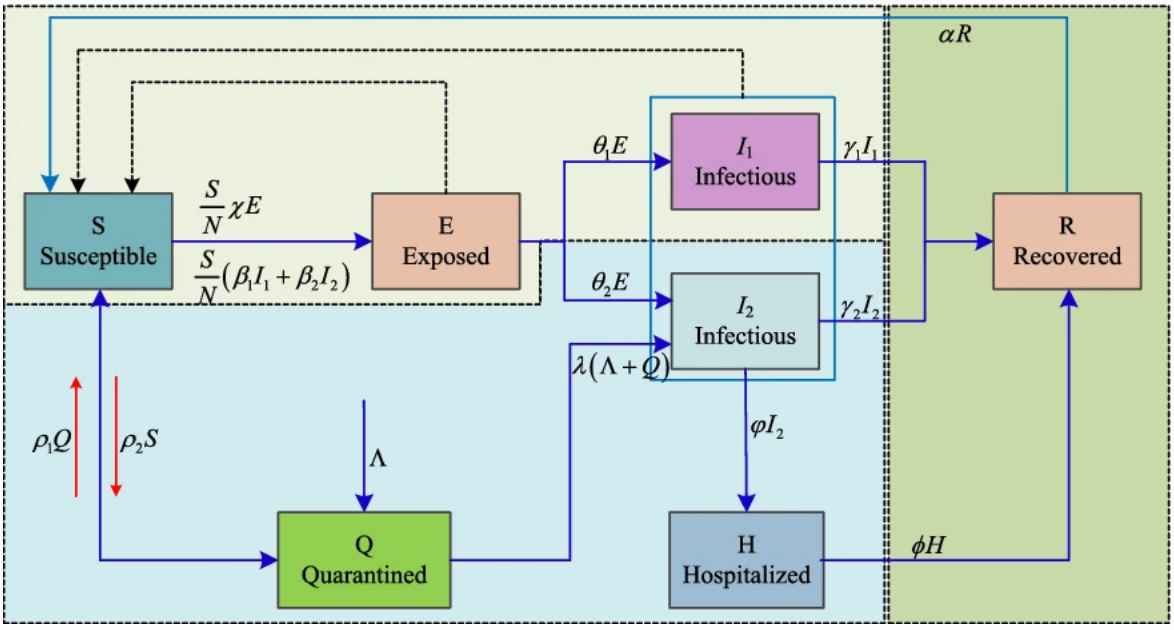
\includegraphics[width=16cm]{../Figures/Model_flowchart.png}
    \caption{Diagrama de flujo del modelo}
    \label{block_diagram}
\end{figure*}


\end{document}
